\documentclass[main.tex]{subfiles}
\begin{document}

\chapter{Kansruimten}
\label{cha:kansruimten}

\begin{de}
  Een \term{stochastisch experiment} is een experiment waarvan de uitkomst op voorhand onbekend is.
\end{de}

\begin{de}
  Het \term{universum} van een stochastisch experiment is de verzameling van alle mogelijke uitkomsten.
\end{de}

\begin{de}
  Een \term{gebeurtenis} van een stochastisch experiment is een deelverzameling van het universum.
\end{de}

\begin{de}
  Een \term{Bernoulli experiment} is een stochastisch experiment met maar twee mogelijke uitkomsten.
\end{de}

\section{Sigma algebra's}

\begin{de}
  \label{de:sigma-algebra}
  Een \term{sigma algebra} of \term{$\sigma$-algebra} $\mathcal{A}$ is een verzameling $\mathcal{A}$ van deelverzamelingen van een \term{universum} $\Omega$ die voldoet aan de volgende drie axioma's.
  \begin{enumerate}
  \item $\Omega \in \mathcal{A}$
  \item $A\in \mathcal{A} \Rightarrow A^{C} \in \mathcal{A}$
  \item $(\forall n\in \mathbb{N}: A_{n} \in \mathcal{A}) \Rightarrow \bigcup_{n\in \mathbb{N}}A_{n} \in \mathcal{A}$
  \end{enumerate}
  De structuur $\Omega,\mathcal{A}$ wordt een \term{meetbare ruimte} genoemd en de verzamelingen in $\mathcal{A}$ noemen we \term{gebeurtenissen}.
\end{de}

\begin{st}
  \label{st:lege-verzameling-in-sigma-algebra}
  Zij $\mathcal{A}$ een sigma-algebra.
  \[ \emptyset \in \mathcal{A} \]

  \begin{proof}
    De eerste twee axioma's, samen met $\Omega^{C} = \emptyset$ geeft de stelling. 
  \end{proof}
\end{st}

\begin{st}
  \label{st:sigma-algebra-eindige-unie}
  Zij $\mathcal{A}$ een sigma-algebra.
  \[ (\forall n\in \{ 1,\dotsc,n \}: A_{n} \in \mathcal{A}) \Rightarrow \bigcup_{n\in \{1,\dotsc,n\}}A_{n} \in \mathcal{A} \]

  \begin{proof}
    We kunnen in het derde axioma de $n+1,...$ gebeurtenissen gelijkstellen aan de lege verzameling om een eindige unie te bekomen.
  \end{proof}
\end{st}

\begin{st}
  \label{st:sigma-algebra-oneindige-doorsnede}
  Zij $\mathcal{A}$ een sigma-algebra.
  \[ (\forall n\in \mathbb{N}: A_{n} \in \mathcal{A}) \Rightarrow \bigcap_{n\in \mathbb{N}}A_{n} \in \mathcal{A} \]

  \begin{proof}
    Het eerste axioma, samen met stelling \ref{st:sigma-algebra-eindige-unie} en de tweede wet van de morgan\stref{st:tweede-wet-van-de-morgan} geeft de stelling.
  \end{proof}
\end{st}

\begin{st}
  Zij $\mathcal{A}$ een sigma-algebra.
  \[ (\forall n\in \{ 1,\dotsc,n \}: A_{n} \in \mathcal{A}) \Rightarrow \bigcap_{n\in \{1,\dotsc,n\}}A_{n} \in \mathcal{A} \]

  \begin{proof}
    We kunnen in stelling \ref{st:sigma-algebra-oneindige-doorsnede} de $n+1,...$ gebeurtenissen gelijkstellen aan het universum om een eindige doorsnede te bekomen.
  \end{proof}
\end{st}

\begin{st}
  Zij $\mathcal{A}$ een sigma-algebra.
  \[ \forall A,B \in \mathcal{A}: A \triangle B \in \mathcal{A} \]

  \begin{proof}
    Het symmetrisch verschil $A \triangle B$ is gelijk aan $(A\cup B) \cap (A \cap B)^{C}$.\stref{st:verschil-verzamelingen-is-doorsnede-complement} \stref{st:symmetrisch-verchil-enkelvoudig-verchil.}
    Neem nu stelling \ref{st:sigma-algebra-eindige-unie}, \ref{st:sigma-algebra-oneindige-doorsnede} en het eerste axioma samen om de stelling te bekomen.
  \end{proof}
\end{st}

\begin{de}
  $\{ \emptyset, \Omega \}$ noemen we de \term{triviale $\sigma$-algebra}.
\end{de}
\begin{de}
  $\Omega,\{ \emptyset, \Omega \}$ noemen we de \term{triviale meetbare ruimte}.
\end{de}

\begin{de}
  \label{de:discrete-sigma-algebra}
  De de machtsverzameling van een universum noemen we de \term{discrete $\sigma$-algebra}.
\end{de}

\begin{tvb}
   De unie van een aantal $\sigma$-algebra's is niet noodzakelijk een $\sigma$-algebra.

   \begin{proof}
     Beschouw de $\sigma$-algebra's $B$ en $C$:
     \[ B = \{ \emptyset , \{0\} , \{1,2\}, \{0,1,2\} \} \quad\text{ en }\quad \{ \emptyset , \{1\} , \{0,2\}, \{0,1,2\} \} \]
     De unie hiervan is geen $\sigma$-algebra:
     \[ B \cup B = \{ \emptyset, \{0\}, \{1\}, \{0,2\}, \{1,2\}, \{0,1,2\} \} \]
     De unie van $\{0\}$ en $\{1\}$ zit er namelijk niet in.\stref{st:sigma-algebra-eindige-unie}
   \end{proof}
\end{tvb}

\section{Kansmaten}
\label{sec:kansmaten}

\begin{de}
  Zij $\mathcal{A}$ een kansruimten.
  Een \term{kansmaat} is een afbeelding $P:\ \mathcal{A} \rightarrow [0,1] \subset \mathbb{R}$ met de volgende eigenschappen.
  \begin{enumerate}
  \item $P(\Omega) = 1$
  \item $\forall A \in \mathcal{A}:\ P(A) \ge 0$
  \item De \term{aftelbare additiviteit} of \term{$\sigma$-additiviteit}:\\
    Zij $(A_{n})_{n}$ een aftelbaar-oneindige rij van onderling disjuncte verzamelingen.
    \[ P\left( \bigcup_{n\in\mathbb{N}}A_{n} \right) = \sum_{n\in\mathbb{N}}P(A_{n}) \]
  \end{enumerate}
  De structuur $\Omega,\mathcal{A},P$ noemen we een \term{kansruimte}.
\end{de} 

\begin{de}
  Zij $(A_{n})_{n}$ een rij verzamelingen, dan noemen we deze rij ...
  \begin{itemize}
  \item ... \term{stijgend} als $\forall n:\ A_{n}\subseteq A_{n+1}$ geldt: $A_{n}\uparrow$
  \item ... \term{dalend} als $\forall n:\ A_{n}\supseteq A_{n+1}$ geldt: $A_{n}\downarrow$
  \item ... \term{monotoon} als ze stijgend of dalend is.
  \end{itemize}
\end{de}

\begin{de}
  Zij $(A_{n})_{n}$ een stijgende rij verzamelingen: $A_{n} \uparrow$
  \[ \lim_{n\rightarrow \infty}A_{n} = \bigcup_{n\in \mathbb{N}}^{\infty}A_{n} \]
\end{de}

\begin{de}
  Zij $(A_{n})_{n}$ een dalende rij verzamelingen: $A_{n} \downarrow$
  \[ \lim_{n\rightarrow \infty}A_{n} = \bigcap_{n\in \mathbb{N}}^{\infty}A_{n} \]
\end{de}


\begin{st}
  \label{st:kansmaat-eindige-additiviteit}
  Zij $\Omega,\mathcal{A},P$ een kansruimte en $\{ A_{n} \mid n\in \{ 1,\dotsc,N\} \}$ $N$ paarsgewijze disjuncte gebeurtenissen.
  \[ P\left( \bigcup_{n=1}^{N}A_{n}\right) = \sum_{n=1}^{N}P(A_{n}) \]

  \begin{proof}
    Kies voor de $n+1,\dotsc$ gebeurtenissen in het derde axioma van een kansmaat telkens de lege gebeurtenis om de stelling te bekomen.
  \end{proof}
\end{st}

\begin{st}
  Zij $\Omega,\mathcal{A},P$ een kansruimte.
  \[ \forall A \in \mathcal{A}:\ P(A^{C}) = 1 - P(A) \]

  \begin{proof}
    Begin met de uitdrukking $\Omega = A \cup A^{C}$.
    Pas nu stelling \ref{st:kansmaat-eindige-additiviteit} toe:
    \[
    \begin{array}{rl}
      P(\Omega) &= P(A) + P(A^{C})\\
      1         &= P(A) + P(A^{C})\\
      P(A^{C})  &= 1-P(A)
    \end{array}
    \]
  \end{proof}
\end{st}

\begin{gev}
  $P(\emptyset) = 0$
\end{gev}

\begin{st}
  Zij $\Omega,\mathcal{A},P$ een kansruimte en $(A_{n})_{n}$ een monotone rij verzamelingen.
  \[ P\left( \lim_{n\rightarrow \infty}A_{n} \right) = \lim_{n\rightarrow \infty}P(A_{n}) \]

  \begin{proof}
    We bewijzen de stelling voor een stijgende rij verzamelingen $(A_{n})_{n}$.
    Herschrijven we het linker lid, dan krijgen we de volgende unie:
    \[
    \begin{array}{rll}
      P\left( \lim_{n\rightarrow \infty}A_{n} \right) &= P \left( \bigcup_{n\in \mathbb{N}}^{\infty}A_{n} \right)\\
                                                &= P \left( A_{1} \bigcup_{n=2}^{\infty}(A_{n} \setminus A_{n-1}) \right)\\
                                                &= P(A_{1}) + \sum_{n=1}^{\infty}P(A_{n}\setminus A_{n-1})\\
                                                &= P(A_{1}) + \lim_{N \rightarrow \infty}\sum_{n=1}^{N}(P(A_{n}) - P(A_{n-1}))\\
                                                &= P(A_{1}) + \lim_{N \rightarrow \infty}\sum_{n=1}^{N}P(A_{n}) - P(A_{1}) &= \lim_{n\rightarrow \infty}P(A_{n})\\
    \end{array}
    \]
  \end{proof}
\end{st}

\begin{ei}
  Zij $\Omega,\mathcal{A},P$ een kansruimte.
  \[ \forall A,B \in \mathcal{A}:\ P(B) = P(B \cap A) + P(B \cap A^{C}) \]

  \begin{proof}
    $P(B) = P((B \cap A) \cup (B \cap A^{C})) = P(B \cap A) + P(B \cap A^{C})$ met $(B \cap A)$ en $(B \cap A^{C})$ disjunct.\stref{st:kansmaat-eindige-additiviteit}
  \end{proof}
\end{ei}

\begin{ei}
  Zij $\Omega,\mathcal{A},P$ een kansruimte.
  \[ \forall A,B \in \mathcal{A}:\ P(A \cup B) = P(A) + P(B) - P(A \cap B) \]

  \begin{proof}
    \[
    \begin{array}{rll}
      P(A \cup B) &= P((A \cap B^{C}) \cup (A \cap B) \cup (A^{C}\cap B)) \\
                  &= P(A \cap B^{C})+P(A \cap B) +P(A^{C}\cap B)\\
                  &= (P(A \cap B^{C})+P(A \cap B)) +((P(A^{C}\cap B)+P(A \cap B)) -P(A\cap B) \\
                  &= P(A)+P(B) -P(A\cap B)\\
    \end{array}
    \]
  \end{proof}
\end{ei}


\begin{ei}
  \label{ei:kansmaat-verschil}
  Zij $\Omega,\mathcal{A},P$ een kansruimte.
  \[ \forall A,B \in \mathcal{A}:\ P(A \setminus B) = P(A\cup B) - P(B) \]

  \begin{proof}
    $P(A \cup B) = P(B \cup (A\setminus B)) = P(B) + P(A \setminus B)$
  \end{proof}
\end{ei}

\begin{ei}
  \label{ei:kansmaat-kans-deelverzameling-kleiner}
  Zij $\Omega,\mathcal{A},P$ een kansruimte.
  \[ \forall A,B \in \mathcal{A}:\ A \subseteq B \Rightarrow P(A) \le P(B) \]

  \begin{proof}
    $P(A) = P(B \setminus (B \cap A^{C})) = P(B) - P(B \cap A^{C}) \le P(B)$ vanwege axioma 2 en eigenschap \ref{ei:kansmaat-verschil}.
  \end{proof}
\end{ei}

\begin{ei}
  Zij $\Omega,\mathcal{A},P$ een kansruimte.
  \[ \forall A \in \mathcal{A}:\ P(A) \le 1 \]

  \begin{proof}
    $A$ is steeds een deelverzameling van $\Omega$.
    Gebruik nu eigenschap \ref{ei:kansmaat-kans-deelverzameling-kleiner}.
  \end{proof}
\end{ei}


\section{Traditionele kansruimten}
\label{sec:trad-kansr}

\begin{de}
  De \term{uniforme kansmaat} is een kansmaat die enkel gedefini\"eerd is voor eindige verzamelingen.
  \[ P:\ \mathcal{A} \rightarrow [0,1] \subset \mathbb{R}:\ A \mapsto \frac{|A|}{|\Omega|} \]
\end{de}

\begin{de}
  De \term{discrete kansmaat} (?) is een kansmaat die enkel gedefini\"eerd is voor aftelbare verzamelingen.
  \[ P:\ \mathcal{A} \rightarrow [0,1] \subset \mathbb{R}:\ A \mapsto p_{i} \]
  Hier is het natuurlijk essentieel dat $\sum_{i}p_{i}=1$ geldt. 
\end{de}

\begin{de}
  Zij $\mathcal{C} \subseteq \Omega$ een collectie deelverzamelingen van een universum.
  De $\sigma$-algebra $\sigma(\mathcal{C})$ \term{voortgebracht door} $\mathcal{C}$ is de kleinste $\sigma$-algebra die $\mathcal{C}$ bevat.

  \begin{itemize}
  \item $\sigma(\mathcal{C}$ is een $\sigma$-algebra.
  \item $\mathcal{C} \subseteq \sigma(\mathcal{C})$
  \item Elke $\sigma$-algebra $\mathcal{A}$ met $\mathcal{C} \subseteq \mathcal{A}$ omvat $\sigma(\mathcal{C})$.
  \end{itemize}
\end{de}

\begin{st}
  De $\sigma$-algebra opgespannen door een collectie deelverzamelingen van een universum is uniek.

  \begin{proof}
    Als er immers nog een (even kleine) sigma algebra zou zijn die aan de voorwaarde voldoet dan zouden ze gelijk zijn volgens de derde eigenschap.
  \end{proof}
\end{st}

\begin{ei}
  Voor elke collectie deelverzamelingen $\mathcal{C} \subseteq \Omega$ bestaat $\sigma(C)$.

  \begin{proof}
    Niet constructief bewijs van existentie\\
    Beschouw voor een gegeven collectie deelverzamelingen $\mathcal{C}$ de verzameling $X$:
    \[ X = \{ \mathcal{A} \subseteq \mathcal{P}(\Omega) \mid \mathcal{A} \text{ is een $\sigma$-algebra.} \wedge \mathcal{C} \subseteq \mathcal{A} \} \]
    Merk allereerst op dat $X$ niet leeg is omdat $\mathcal{P}(\Omega)$ altijd een $\sigma$-algebra is (en $\mathcal{C}$ omvat).\deref{de:discrete-sigma-algebra}
    We moeten nog de kleinste $\sigma$-algebra selecteren uit $X$.
    Bekijk hiervoor $\mathcal{B}$:
    \[ \mathcal{B} = \bigcap_{\mathcal{A} \in X}\mathcal{A} \]
    $\mathcal{B}$ omvat nu zeker $\mathcal{C}$ omdat $C$ een deel is van elke $\mathcal{A} \in X$.
    We tonen nu aan dat $\mathcal{B}$ een $\sigma$-algebra is.
\extra{bewijs dit.}
    \begin{itemize}
    \item $\Omega \in \mathcal{A}$
    \item $A \in \mathcal{A} \Rightarrow A^{C} \in \mathcal{A}$
    \item $(\forall n\in \mathbb{N}: A_{n}\in \mathcal{A}) \Rightarrow \bigcup_{n\in \mathbb{N}} A_{n} \in \mathcal{A}$
    \end{itemize}
  \end{proof}
\end{ei}

\begin{de}
  De \term{Borel $\sigma$-algebra op $\mathbb{R}$} is de $\sigma$-algebra voortgebracht door $\mathcal{C}$:
  \[ \{ ]-\infty,a] \mid a \in \mathbb{R} \} \]  
  \[ \{ \interval{a}{b} \mid a,b\in \mathbb{R} \} \]  
\end{de}

\begin{st}
  Het \term{theorema van Vitali}\\
  Er bestaat geen uniforme kansverdeling op het interval $[0,1]$.
\zb
\end{st}

\section{Voorwaardelijke kans en onafhankelijkheid}
\label{sec:voorwaardelijke-kans-en-onafhankelijkheid}

\subsection{Voorwaardelijke kans}
\label{sec:voorwaardelijke-kans}

\begin{de}
  \label{de:voorwaardelijke-kans} 
  Zij $\Omega,\mathcal{A},P$ een kansruimte.
  De \term{voorwaardelijke kans} of \term{conditionele kans} van een gebeurtenis $A$ gegeven een gebeurtenis $B$ (met $P(B) \neq 0$) is $P(A|B)$.
  \[ P(A|B) = \frac{P(A\cap B)}{P(B)} \]
\end{de}

\begin{ei}
  Zij $\Omega,\mathcal{A},P$ een kansruimte.
  \[ \forall A \in \mathcal{A}: P(A|A) = 1 \]

  \begin{proof}
    \[ \forall A \in \mathcal{A}: P(A|A) = \frac{P(A \cap A)}{P(A)} = \frac{P(A)}{P(A)} = 1 \]
  \end{proof}
\end{ei}

\begin{ei}
  \label{ei:gebeurtenis onafhankelijk van universum}
  Zij $\Omega,\mathcal{A},P$ een kansruimte.
  Elke gebeurtenis is onafhankelijk van zijn universum.
  \[ \forall A \in \mathcal{A}: P(A|\Omega) = P(A) \]

  \begin{proof}
    \[ \forall A \in \mathcal{A}: P(A|\Omega) \frac{P(A \cap A)}{P(A)} = \frac{P(A)}{P(\Omega)} = \frac{P(A)}{1} = P(A)\]
  \end{proof}
\end{ei}

\begin{st}
  Zij $\Omega,\mathcal{A},P$ een kansruimte en $B$ een gebeurtenis in $\mathcal{A}$ met kans groter dan nul.
  De functie $P_{B}$ is een kansmaat.
  \[ P_{B}:\ \mathcal{A} \rightarrow [0,1] \subset \mathbb{R}:\ A \mapsto P(A|B) \]

  \begin{proof}
    We gaan elke definierende eigenschap van een kansmaat af.
    \begin{itemize}
    \item $P_{B}(\Omega) = P(\Omega|B) = \frac{P(\Omega \cap B)}{P(\Omega)} = \frac{P(B)}{P(B)} = 1$
    \item $\forall A \in \mathcal{A}:\ P_{B}(A) = \frac{P(A\cap B)}{P(B)} \ge 0$
    \item Zij $(A_{n})_{n}$ een paarsgewijs disjuncte rij van gebeurtenissen in $\mathcal{A}$.
      \[
      \begin{array}{rl}
        P_{B}\left( \bigcup_{n=1}^{\infty} A_{n} \right)
        &= \frac{P\left(\left( \bigcup_{n=1}^{\infty} A_{n} \right) \cap B \right)}{P(B)}\\
        &= \frac{P\left(\bigcup_{n=1}^{\infty} (A_{n} \cap B)\right)}{P(B)}\\
        &= \frac{\sum_{n=1}^{\infty}P\left(A_{n} \cap B\right)}{P(B)}\\
        &= \sum_{n=1}^{\infty}P_{B}(A_{n})\\
      \end{array}
      \]
    \end{itemize}
  \end{proof}
\end{st}

\subsection{Kettingregel}
\label{sec:kettingregel}

\begin{st}
  Zij $\Omega,\mathcal{A},P$ een kansruimte.
  Zij $\{ A_{1}, A_{2}, \dotsc, A_{k}\}$ meer dan \'e\'en gebeurtenis in $\mathcal{A}$.

  \[
  P\left(\bigcap_{i=1}^{k}A_{i}\right)
  = \prod_{i=1}^{k}P\left(A_{i}\mid\bigcap_{j=1}^{i-1}A_{j}\right)
  \]
  \[
  P(A_{1}\cap A_{2} \dotsb A_{k}
  = P(A_{1})P(A_{2}|A_{1})P(A_{3}|A_{1}\cap A_{2}) \dotsb P(A_{k}|A_{1}\cap A_{2}\cap \dotsc \cap A_{k-1})
  \]

  \begin{proof}
    Bewijs door volledige inductie op $\mathbb{N} \setminus \{0,1\}$:
    \begin{itemize}
    \item De stelling geldt voor $k=2$ vanuit de definitie van voorwaardelijke kans:\deref{de:voorwaardelijke-kans} 
      \[  P(A_{1}|A_{2}) = \frac{P(A_{1}\cap A_{2})}{P(A_{2})} \Rightarrow P(A_{1} \cap A_{2}) = P(A_{1}) P(A_{2}|A_{1}) \]
    \item Uit de stelling voor $k=n$ volgt dat de stelling geldt voor $k=n+1$:\\
      We gebruiken hier het basisgeval.
      \[ 
      \begin{array}{rl}
        P\left(\bigcap_{i=1}^{n+1}A_{k}\right)
        &= P\left(\left(\bigcap_{i=1}^{n}A_{p}\right) \cap A_{n+1} \right)\\
        &= P\left(A_{n+1} | \left(\bigcap_{i=1}^{n}A_{p}\right) \right) P\left(\bigcap_{i=1}^{n+1}A_{k}\right)\\
        &= \prod_{i=1}^{n}P\left(A_{i}\mid\bigcap_{j=1}^{i-1}A_{j}\right) P\left(\bigcap_{i=1}^{n+1}A_{k}\right)\\
        &= \prod_{i=1}^{n+1}P\left(A_{i}\mid\bigcap_{j=1}^{i-1}A_{j}\right)\\
      \end{array}
      \]
    \end{itemize}
  \end{proof}
\end{st}

\subsection{Wet van de totale kans}
\label{sec:wet-van-de}

\begin{st}
  Zij $\Omega,\mathcal{A},P$ een kansruimte en $X$ een partitie van $\Omega$ waarin $\forall A \in X:\ P(A) > 0$ geldt.
  \[ \forall B \in A:\ P(B) = \sum_{A\in X}P(A)P(B|A) \]
  \begin{proof}
    \[
    \begin{array}{rl}
      \sum_{A\in X}P(A)P(B|A)
      &= \sum_{A\in X}\frac{P(A)P(B \cap A)}{P(A)}\\
      &= \sum_{A\in X} P(B \cap A)\\
      &= P(\cup_{A\in X}(B \cap A))\\
      &= P(B \cap \cup_{A\in X}(A))\\
      &= P(B \cap \Omega) = P(B)\\
    \end{array}
    \]
  \end{proof}
\end{st}

\subsection{Stelling van Bayes}
\label{sec:stelling-van-bayes}

\begin{st}
  \label{st:bayes}
  Zij $\Omega,\mathcal{A},P$ een kansruimte en $X$ een partitie van $\Omega$ waarin $\forall A \in X:\ P(A) > 0$ geldt.
  Zij $B$ een gebeurtenis in $\mathcal{A}$ met $P(B) > 0$.
  \[ \forall A\in X:\ P(A|B) = \frac{P(A)P(B|A)}{\sum_{C\in X}P(C)P(B|C)} \]
  \begin{proof}
    \[
      \begin{array}{rl}
        \frac{P(A)P(B|A)}{\sum_{C\in X}P(C)P(B|C)}
        &= \frac{P(A)P(B|A)}{P(B)}\\
        &= \frac{P(A \cap B)}{P(B)} = P(A|B)\\
      \end{array}
    \]
  \end{proof}
\end{st}

\subsection{Handige rekenregels}
\label{sec:handige-rekenregels}

\begin{st}
  Zij $\Omega,\mathcal{A},P$ een kansruimte.
  \[
  \forall A,B \in \mathcal{A}: P(A|B) = \frac{P(A)}{P(B)}P(B|A)
  \]
  
  \begin{proof}
    \[
    \begin{array}{rl}
      P(A|B)
      &= \frac{P(A\cap B)}{P(B)}\\
      &= \frac{P(A)P(A\cap B)}{P(B)P(A)}\\
      &= \frac{P(A)}{P(B)}\frac{P(A\cap B)}{P(A)}\\
      &= \frac{P(A)}{P(B)}P(B|A)\\
    \end{array}
    \]
  \end{proof}
\end{st}

\begin{st}
  \label{st:rekenregel-afhankelijkheid-partitie}
  Zij $\Omega,\mathcal{A},P$ een kansruimte en $X$ een partitie van $\Omega$ waarin $\forall A \in X:\ P(A) > 0$ geldt.
  Zij $X$ een gebeurtenis in $\Omega$.
  \[ \sum_{A \in X}P(A|X) = 1 \]

  \begin{proof}
    \[
    \begin{array}{rl}
      \sum_{A \in X}P(A|X)
      &= \sum_{A \in X}\frac{P(A\cap X)}{P(X)}\\
      &= \frac{\sum_{A \in X}P(A \cap X)}{P(X)}\\
      &= \frac{P\left(\bigcup_{A \in X}A \cap X\right)}{P(X)}\\
      &= \frac{P\left(\bigcup_{A \in X}A\right) \cap X}{P(X)}\\
      &= \frac{P( \Omega \cap X)}{P(X)}\\
      &= \frac{P(X)}{P(X)}\\
      &= 1
    \end{array}
    \]
  \end{proof}
\end{st}

\begin{st}
  Zij $\Omega,\mathcal{A},P$ een kansruimte en $(A_{i})_{n}$ een rij in $\mathcal{A}$.
  \[ P\left(  \bigcup_{n}A_{n}\right) = P(A_{1}) + \sum_{n>1}P\left( A_{n} \cap\bigcap_{i=1}^{n-1} A_{i}^{C}\right)\]

  \begin{proof}
    We bewijzen, nog sterker, dat de bewering geldt voor elke aftelbare verzameling $A_{i}\in \mathcal{A}$ in $\mathcal{A}$.\\
    Bewijs door volledige inductie op $\mathbb{N}$:
    \begin{itemize}
    \item De stelling geldt voor $n=1$
      \[ P(A_{1} \cup A_{2}) = P(A_{1} \cup \left(A_{1}^{C} \cap A_{2}\right) = P(A_{1}) + P(A_{1}^{C} \cap A_{2}) \]
    \item Uit de stelling voor $k=n$ volgt de stelling voor $k+1$.
      \[
      P\left( \bigcup_{i=1}^{n+1}A_{i}\right)
      = P\left( A_{n+1} \cup \bigcup_{i=1}^{n}A_{i}\right) 
      = P\left(\left(\bigcup_{i=1}^{n} A_{i}\right)^{C}\cap A_{n+1}\right) + P\left(\bigcup_{i=1}^{n}A_{i}\right) 
      = P(A_{1}) + \sum_{n>1}P\left( A_{n} \cap\bigcap_{i=1}^{n-1} A_{i}^{C}\right)
      \]
    \end{itemize}
  \end{proof}
\end{st}

\subsection{Onafhankelijkheid}
\label{sec:onafhankelijkheid}
\begin{de}
  Zij $\Omega,\mathcal{A},P$ een kansruimte.
  We noemen twee gebeurtenissen $A$ en $B$ uit $\mathcal{A}$ \term{onafhankelijk} als het volgende geldt over hun kans:
  \[ P(A\cap B) = P(A) \cdot P(B) \]
\end{de}

\begin{de}
  Zij $\Omega,\mathcal{A},P$ een kansruimte en $A$ en $B$ twee afhankelijke gebeurtenissen uit $\mathcal{A}$ dan noemen we de afhankelijkheid ...
  \begin{itemize}
  \item ... \term{positieve afhankelijkheid} als $P(A \cap B) > P(A)P(B)$ geldt.
  \item ... \term{negatieve afhankelijkheid} als $P(A \cap B) < P(A)P(B)$ geldt.
  \end{itemize}
\end{de}

\begin{st}
  Zij $\Omega,\mathcal{A},P$ een kansruimte en $A$ en $B$ twee onafhankelijke gebeurtenissen uit $\mathcal{A}$.
  \[ P(A|B) = P(A) \]
  
  \begin{proof}
    \[ P(A|B) = \frac{P(A \cap B)}{P(B)} = \frac{P(A) \cdot P(B)}{P(B)} = P(A) \]
  \end{proof}
\end{st}

\begin{st}
  Zij $\Omega,\mathcal{A},P$ een kansruimte en $A$ en $B$ twee afhankelijke gebeurtenissen uit $\mathcal{A}$, dan zijn er twee mogelijkheden:
  \begin{itemize}
  \item $A$ en $B$ zijn positief afhankelijk: $P(A|B) > P(A)$.
  \item $A$ en $B$ zijn negatief afhankelijk: $P(A|B) < P(A)$.
  \end{itemize}
\end{st}

\begin{de}
  Een verzameling gebeurtenissen noemen we \term{paarsgewijs onafhankelijk} als elke twee gebeurtenissen onafhankelijk zijn.
\end{de}

\begin{de}
  Een eindige verzameling gebeurtenissen $X$ noemen we \term{onderling onafhankelijk} als het volgende geldt:
  \[ \forall Y\in \mathcal{P}(X):\ P\left( \bigcap_{A\in Y}A \right) = \prod_{A\in Y}P(A) \]
\end{de}

\begin{ei}
  Een onderling onafhankelijke verzameling gebeurtenissen is ook zeker paarsgewijs onafhankelijk.
\extra{bewijs}
\end{ei}

\begin{de}
  Een oneindige verzameling gebeurtenissen $X$ noemen we \term{onderling onafhankelijk} als elke eindige deelverzameling gebeurtenissen onderling onafhankelijk is.
\end{de}

\subsection{Systeembetrouwbaarheid}
\label{sec:syst}

\begin{figure}[H]
  \caption{Een serieel systeem}
  \centering
    \includegraphics[width=0.5\textwidth]{assets/systeem-serieel.png}
\end{figure}

\begin{figure}[H]
  \caption{Een parallel systeem}
  \centering
    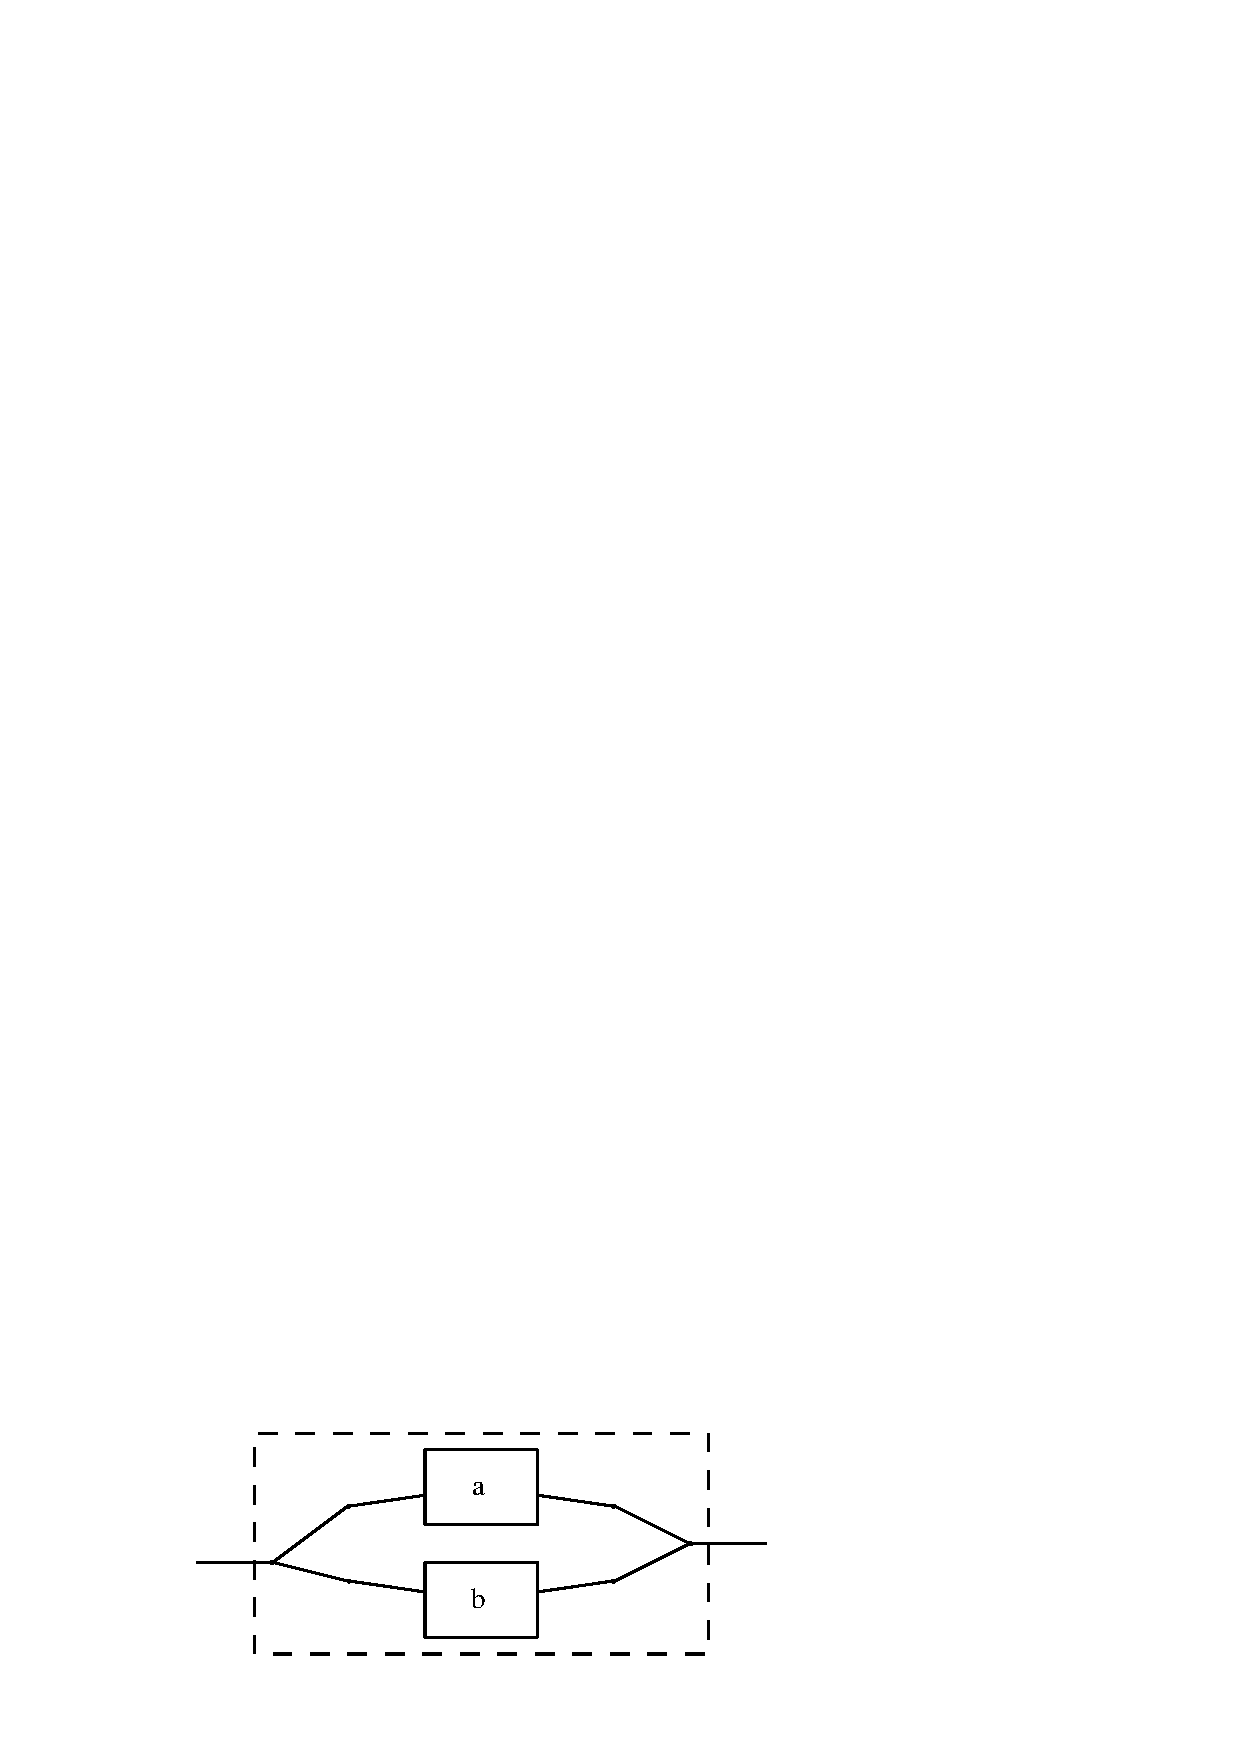
\includegraphics[width=0.5\textwidth]{assets/systeem-parallel.png}
\end{figure}

\begin{de}
  Een \term{serieel systeem} is een systeem met twee componenten dat werk als en slechts als beide componenten werken.
\end{de}

\begin{st}
  In een serieel systeem $S$ met componenten $A$ en $B$ met respectievelijke faalkansen $p_{A}$ en $p_{B}$ is de kans $p_{S}$ dat het systeem werkt als volgt.
  \[ p_{S} = p_{A} + p_{B} -p_{A}p_{B} \]
\TODO{bewijs p 23}
\end{st}

\begin{de}
  Een \term{parallel systeem} is een systeem met twee componenten dat werk als en slechts als \'e\'en van beide componenten werkt.
\end{de}

\begin{st}
  In een parallel systeem $S$ met componenten $A$ en $B$ met respectievelijke faalkansen $p_{A}$ en $p_{B}$ is de kans $p_{S}$ dat het systeem werkt als volgt.
  \[ p_{S} = p_{A}p_{B} \]
\TODO{bewijs p 24}
\end{st}


\end{document}

%%% Local Variables:
%%% mode: latex
%%% TeX-master: t
%%% End:
